\documentclass[a4paper,11pt]{article}

\usepackage{indentfirst}
\usepackage{graphicx}
\usepackage{subcaption}
\usepackage{float}
\usepackage{chngcntr,tocloft}
\usepackage{listings}
\usepackage{comment}
\usepackage{fancyhdr}

\counterwithin*{figure}{section}
\counterwithin*{figure}{subsection}
\counterwithin*{figure}{subsubsection}

\addtolength{\cftfignumwidth}{2em}

\renewcommand{\thefigure}{%
  \ifnum\value{subsection}=0
    \thesection.\arabic{figure}%
  \else
    \ifnum\value{subsubsection}=0
      \thesubsection.\arabic{figure}%
    \else
      \thesubsubsection.\arabic{figure}%
    \fi
  \fi
}

\begin{document}

\begin{titlepage}
	\centering
	{\scshape\LARGE Warsaw University of Technology \par}
	\vspace{1cm}
	{\scshape\Large Faculty of Power and Aeronautical Engineering\par}
	\vspace{3.5cm}
	{\huge\bfseries Influence of air inlet velocity on temperature and thrust for various mixtures\par}
	\vspace{2cm}
	{\Large\ Jeremi Lewandowski, Patryk Ślusarski, Kacper Walczak\par}
	\vfill
	Computational Methods in Combustion\par

	\vfill

% Bottom of the page
	{\large June 2020\par}
\end{titlepage}

\newpage
\tableofcontents

\newpage

\section{Introduction}
The aim of the project was to investigate the effect of inlet speed on combustion and thrust for various fuel mixtures using the Cantera package. The model uses simplified inlet, combustion chamber and exhaust nozzle. As an igniter radical hydrogen atoms were used. 9 various fuel mixtures were taken into account in calculations:
\begin{enumerate}
	\item Methane (1 mol)  -air mixture
	\item Ethane (1 mol) - air mixture
	\item Propane (1 mol) - air mixture
	\item Hydrogen (1 mol) - air mixture
	\item Methane (1 mol) - ethane (0.4 mol) - air mixture
	\item Methane (2 mol) - propane (1 mol) - air mixture
	\item Ethane (1 mol) - hydrogen (0.5 mol) - air mixture
	\item Propane (1 mol) - hydrogen (0.1 mol) - air mixture
	\item Methane (1 mol) - ethane (0.4 mol) - propane (0.2 mol) - air mixture
\end{enumerate}
For each mixture calculations were performed in following conditions:
\begin{enumerate}
  \item Air parameters at 0 m above sea level.
  \item Combustion chamber with a volume of 0.5 $m^3$
  \item The maximum air speed is 7 Mach.
\end{enumerate}
Estimated calculations of thrust in jet engines are often based on empiric data of combustion heat. The idea of injecting radical hydrogen atoms into combustion chamber to initialize combustion comes from Cantera combustor.py example.
\newpage
\section{Mathematical model}
The stoichiometric reaction of complete combustion of ours combustible mixtures in air are as follow:
\begin{itemize}
\item Methane\\
$$CH_4+2(O_2+3,76N_2) ->CO_2+2H_2O+7,52N_2$$
$$A/F=9,52$$
\item Ethane\\
$$C_2H_6+\frac{7}{2}(O_2+3,76N_2)->2CO_2+3H_2O+13,16N_2$$
$$A/F=16,66$$
\item Propane\\
$$C_3H_6+5(O_2+3,76N_2)->3CO_2+4H_2O+18,8N_2$$
$$A/F=23,8$$
\item Hydrogen\\
$$H_2+0,5(O_2+3,76N_2)->H_2O+1,88N_2$$
$$A/F=2,38$$
\end{itemize}

The equivalence ratio was set to 1.\\


Calculations consisted of 3 phases: 
\begin{enumerate}
\item[1]Air parameters were calculated according to specified Mach number 
\item[2]Air, fuel and igniter were added to combustion chamber filled initially with air 
\item[3]Steady-state temperature of methane combustion is used to calculate thrust
\end{enumerate}
First,  velocity of air was calculated according to Mach number and speed of sound:
$$v=M*a=M*\sqrt{\kappa*R*T_0}$$
where 
$$\kappa=\frac{c_v}{c_p}$$
Then the air was set to a higher enthalpy caused by supersonic flow according to $$h=h_0+\frac{v^2}{2}$$
Total pressure of air 
$$p=p_0*{\left(\frac{T}{T_0}\right)}^{\frac{\kappa}{\kappa-1}}$$
Mass of air flowing through the ’combustion chamber’ was set to 
$$m_a\left[\frac{kg}{m}\right]=A/F*\rho_a*A$$
Mass of the fuel
$$m_f=\frac{m_a*\phi}{A/F}$$
where $$\phi=1-equivalence\ ratio $$
Area was set to $0,05 m^2$.
\\
Total mass flow ratio is as follows.
$$m=m_a+m_f$$
Velocity of outlet air was calculated as 
$$v_e\left[\frac{m}{s}\right]=\sqrt{2*c_p*T_0*\left(1-\frac{T}{T_0}\right)}$$
And thrust as
$$T\left[N\right]=m*v_e*(v_e-v_0)-\frac{m}{\rho}*(p_e-p_0)$$
Propulsion efficiency
$$\eta=\frac{2}{1+\frac{v_e}{v_0}}$$


\section{Code}

\begin{lstlisting}

import cantera as ct
import math
import numpy as np
import matplotlib.pyplot as plt

A = 0.1


# calculate kappa
def kappa(gas):
    return gas.cp / gas.cv


# return individual gas constant
def R(gas):
    return ct.gas_constant / gas.mean_molecular_weight


# calculate speed of sound
def sound(gas):
    return math.sqrt(kappa(gas) * gas.T * R(gas))


# calculate velocity from speed of sound and Mach number
def vel(M, gas):
    return M * sound(gas)


# calculate exhaust speed from inlet temperature and outlet temperature
def ve(T0, T, gas):
    return math.sqrt(2.0 * gas.cp * T0 * (1 - T / T0))


# calculate thrust
def thrust(v, v0, mdot, gas, p0):
    return mdot * v * (v - v0) - A * (gas.P - p0)


air0 = ct.Solution('air.xml')  # air
gas = ct.Solution('gri30.xml')  # gas model for fuel, exhaust and igniter

# arrays for plotting
mass = []
temp = []
thr = []
thrm = []
effic = []

Mach = np.linspace(0.01, 7.01, 50)  # Mach array

for Ma in Mach:

    # air parameters
    air = ct.Solution('air.xml')

    ta = 300.0
    ha = air.h
    pa = ct.one_atm
    ka = kappa(air)
    da = air.density

    air.TP = ta, pa
    air0.TP = ta, pa

    # velocity, entalphy of inlet air
    v = vel(Ma, air)
    # change entalphy because of air velocity
    h = ha + v ** 2.0 / 2.0
    # set air parameters after entalphy change
    air.HP = h, pa
    # calculate pressure
    p = pa * (air.T / ta) ** (ka / (ka - 1))
    # set air parameters after pressure change
    air.HP = h, p

    # create reservoir for air
    air_in = ct.Reservoir(air)
    air_mw = air.mean_molecular_weight
    air_r = air.density

    # fuel parameters
    tf = 300.0
    pf = ct.one_atm
    xf = 'XX:X.X, XX:X.X'  # fuel mixture

    # create reservoir for fuel
    gas.TPX = tf, pf, xf
    fuel_in = ct.Reservoir(gas)
    fuel_mw = gas.mean_molecular_weight
    fuel_r = gas.density

    # create reservoir for igniter
    gas.TPX = 300.0, ct.one_atm, 'H:1.0'
    igniter = ct.Reservoir(gas)

    # create combustion reactor
    gas.TPX = air.T, air.P, 'O2:0.21, N2:0.79'
    combustor = ct.IdealGasReactor(gas)
    combustor.volume = 0.5

    # create reservoir for exhaust gas
    exhaust = ct.Reservoir(gas)
    # equivalence ratio
    equiv_ratio = 1
    # stoichometric molecular air demand
    st = XX.XX

    air_mdot = A * st * air_r
    fuel_mdot = air_mdot * equiv_ratio / st

    # create flow controllers for air and fuel
    m1 = ct.MassFlowController(fuel_in, combustor, mdot=fuel_mdot)
    m2 = ct.MassFlowController(air_in, combustor, mdot=air_mdot)

    # igniter time dependent mass flow
    fwhm = 0.3
    amplitude = 0.03
    t0 = 2.0
    igniter_mdot = lambda t: amplitude * math.exp(-(t - t0) ** 2 * 4 * math.log(2) / fwhm ** 2)
    m3 = ct.MassFlowController(igniter, combustor, mdot=igniter_mdot)

    # calculate mass flow rate
    mdot = air_mdot + fuel_mdot

    # create valve for combustor outlet
    valve = ct.Valve(combustor, exhaust, K=1.0)

    # simulation
    sim = ct.ReactorNet([combustor])

    t = 0.0
    tk = 4.0

    tempt = []
    time = []
    while (t < tk):
        t = sim.step()
        tempt.append(combustor.T)
        time.append(t)

    # temperature over time plotting
    """
    plt.plot(time, tempt)
    plt.xlabel('time')
    plt.ylabel('temperature')
    plt.axis([0, 4, 250, 3500])
    plt.title('Mach = %.0f' % (Ma-0.01))
    plt.savefig('M '+str('{0:.2f}'.format(Ma-0.01))+'.png')
    plt.close()
    """

    # calculate velocity of outlet gas
    vee = ve(combustor.T, air.T, gas)
    # calculate thrust
    th = thrust(vee, v, mdot, gas, ct.one_atm)
    # calculate engine efficiency
    eff = 2 / (vee / v + 1)

    mdot_v = vee * mdot

    # fill arrays for plotting
    if (th > 0):
        effic.append(eff)
        temp.append(combustor.T)
        mass.append(mdot)
        thr.append(th)
        thrm.append(th / mdot_v)
    else:
        thr.append(None)
        thrm.append(None)
        mass.append(None)
        temp.append(None)
        effic.append(None)

# plot results and save to .png
names = {'Temperature': temp, 'Thrust': thr, 'Thrust over mass flow rate': thrm, 'Mass flow rate': mass,
         'Efficiency': effic}

for i in names:
    plt.plot(Mach, names[i])
    plt.xlabel('Mach Number')
    plt.ylabel('%s' % (i))
    plt.savefig(i + ' over Mach.png')
    plt.close()

\end{lstlisting}
\newpage


\section{Results}
For each mixture the results of simulations are shown on the plots. 
\subsection{Methane - air mixture}
	\begin{figure}[H]
		\centering
       		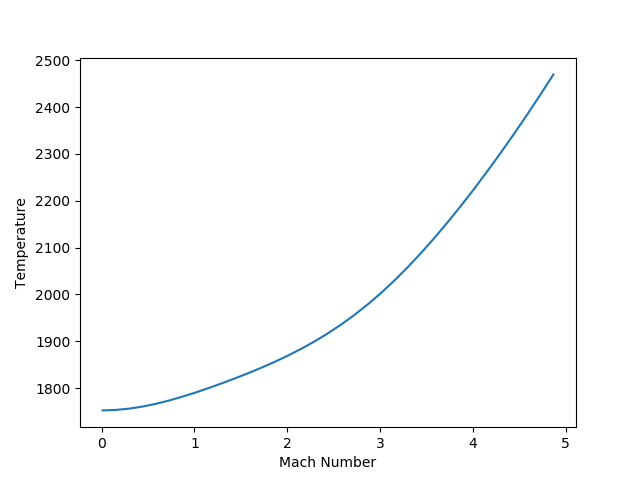
\includegraphics[width=0.9\textwidth]{metan_pow(1mol)/Temperature_over_Mach.png}
       		\caption{Temperature over Mach number for methane-air mixture}
	\end{figure}
	\begin{figure}[H]
		\centering
		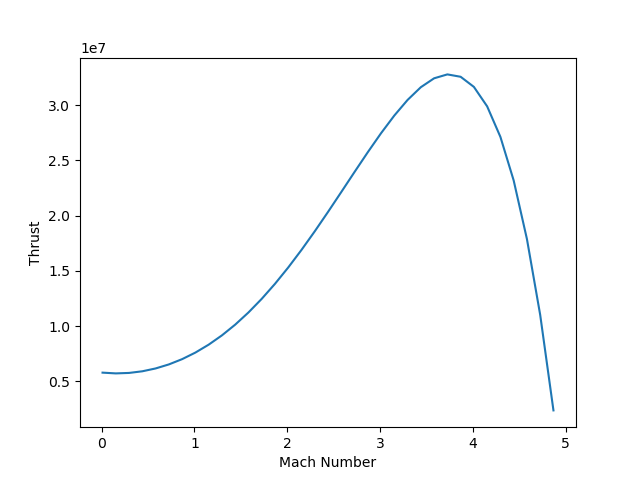
\includegraphics[width=0.9\textwidth]{metan_pow(1mol)/Thrust_over_Mach.png}
       		\caption{Thrust over Mach number for methane-air mixture}
	\end{figure}
	\begin{figure}[H]
		\centering
		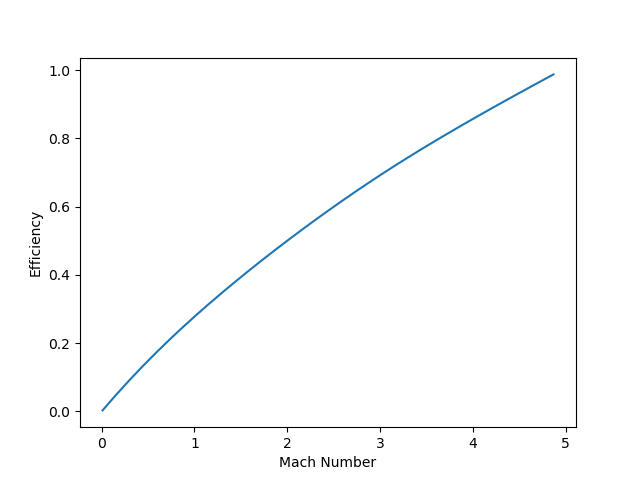
\includegraphics[width=0.9\textwidth]{metan_pow(1mol)/Efficiency_over_Mach.png}
       		\caption{Efficiency over Mach number for methane-air mixture}
	\end{figure}
	\begin{figure}[H]
		\centering
		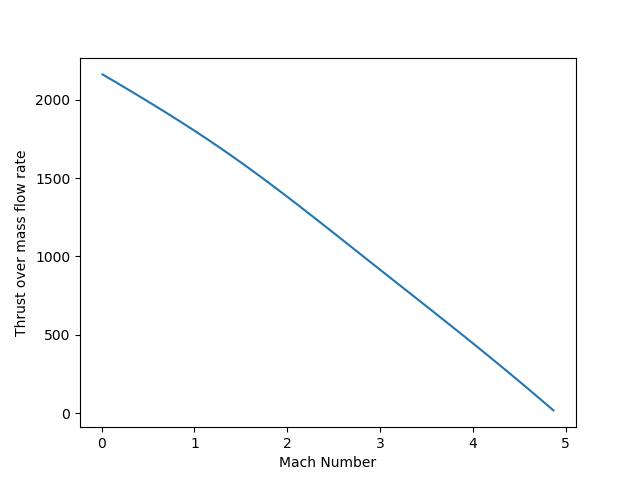
\includegraphics[width=0.9\textwidth]{metan_pow(1mol)/Thrust_over_mass_flow_rate_over_Mach.png}
       		\caption{Thrust over mass flow rate over Mach number for methane-air mixture}
	\end{figure}
	\begin{figure}[H]
		\centering
		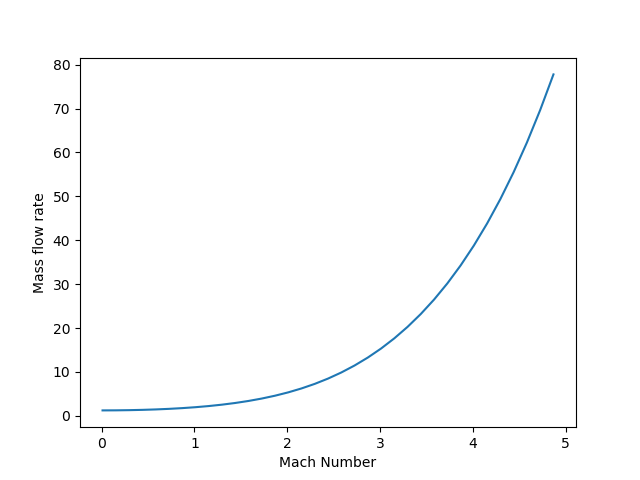
\includegraphics[width=0.9\textwidth]{metan_pow(1mol)/Mass_flow_rate_over_Mach.png}
       		\caption{Mass flow rate over Mach number for methane-air mixture}
	\end{figure}
\subsection{Ethane - air mixture}
	\begin{figure}[H]
		\centering
       		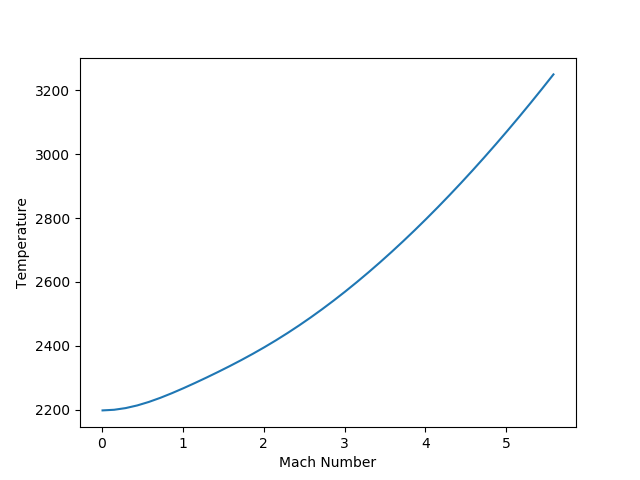
\includegraphics[width=0.9\textwidth]{etan_pow(1mol)/Temperature_over_Mach.png}
       		\caption{Temperature over Mach number for ethane-air mixture}
	\end{figure}
	\begin{figure}[H]
		\centering
		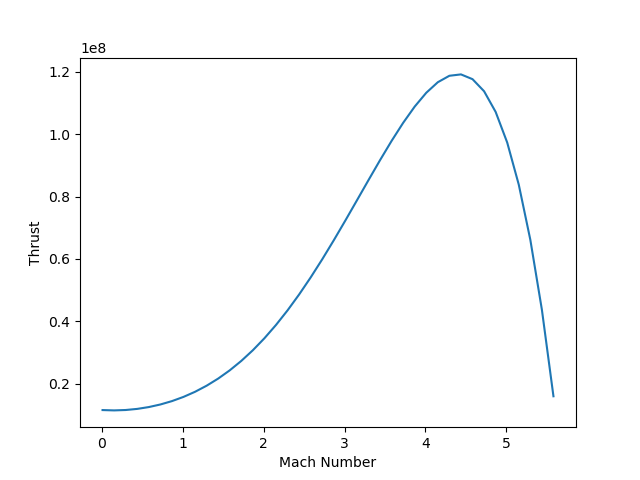
\includegraphics[width=0.9\textwidth]{etan_pow(1mol)/Thrust_over_Mach.png}
       		\caption{Thrust over Mach number for ethane-air mixture}
	\end{figure}
	\begin{figure}[H]
		\centering
		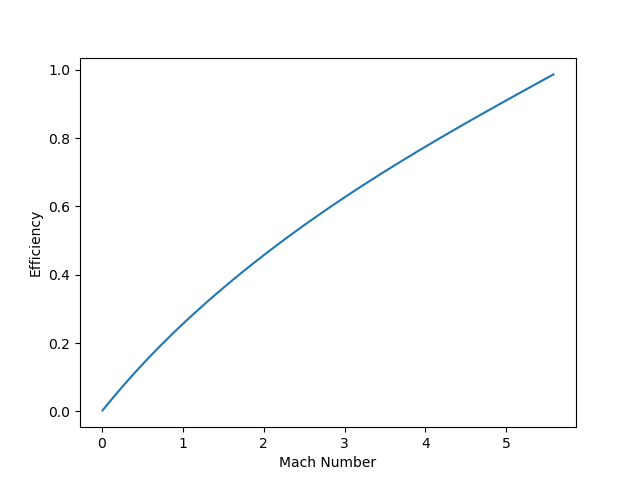
\includegraphics[width=0.9\textwidth]{etan_pow(1mol)/Efficiency_over_Mach.png}
       		\caption{Efficiency over Mach number for ethane-air mixture}
	\end{figure}
	\begin{figure}[H]
		\centering
		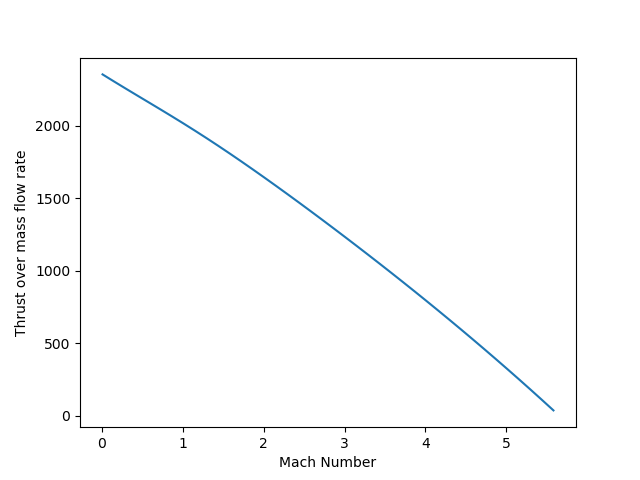
\includegraphics[width=0.9\textwidth]{etan_pow(1mol)/Thrust_over_mass_flow_rate_over_Mach.png}
       		\caption{Thrust over mass flow rate over Mach number for ethane-air mixture}
	\end{figure}
	\begin{figure}[H]
		\centering
		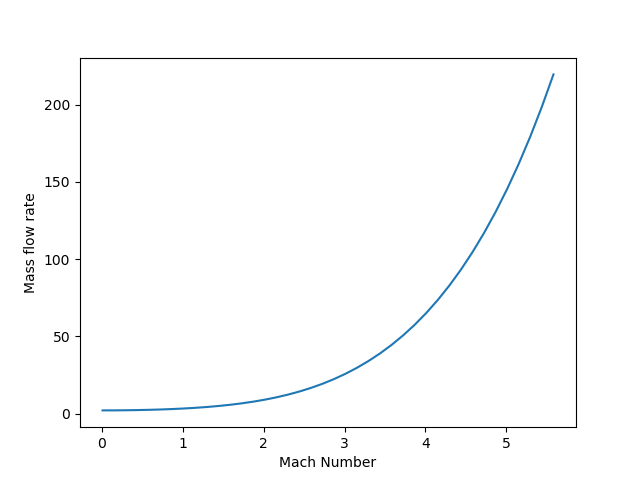
\includegraphics[width=0.9\textwidth]{etan_pow(1mol)/Mass_flow_rate_over_Mach.png}
       		\caption{Mass flow rate over Mach number for ethane-air mixture}
	\end{figure}
\subsection{Propane - air mixture}
	\begin{figure}[H]
		\centering
       		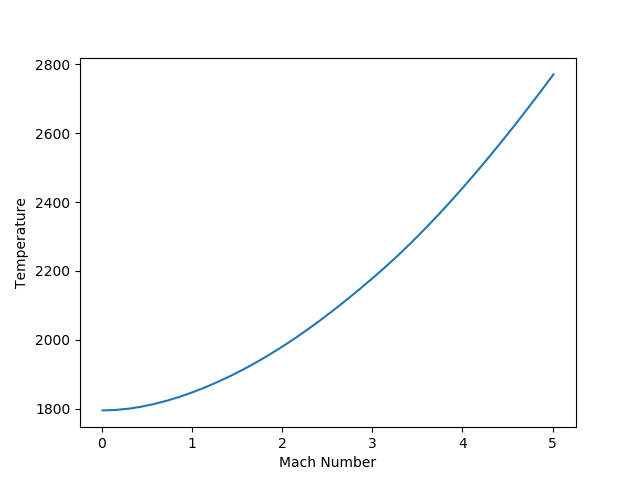
\includegraphics[width=0.9\textwidth]{propan_pow(1mol)/Temperature_over_Mach.png}
       		\caption{Temperature over Mach number for propane-air mixture}
	\end{figure}
	\begin{figure}[H]
		\centering
		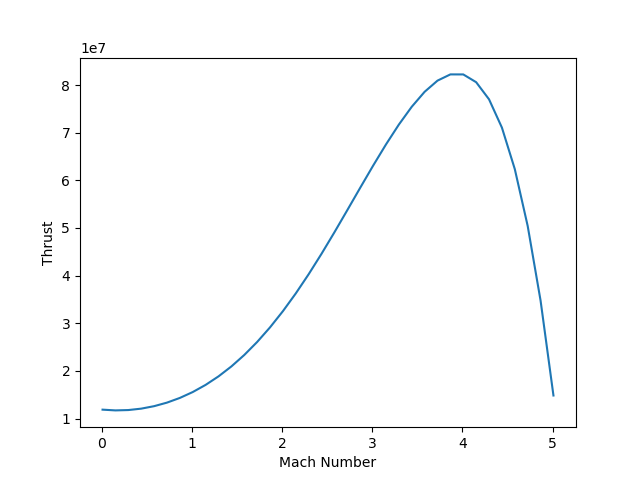
\includegraphics[width=0.9\textwidth]{propan_pow(1mol)/Thrust_over_Mach.png}
       		\caption{Thrust over Mach number for propane-air mixture}
	\end{figure}
	\begin{figure}[H]
		\centering
		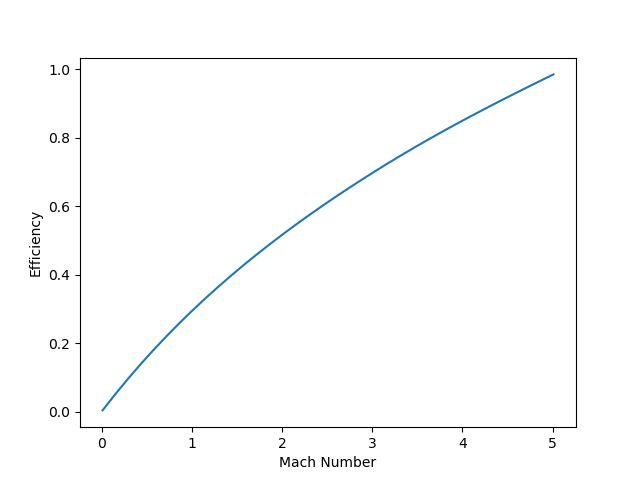
\includegraphics[width=0.9\textwidth]{propan_pow(1mol)/Efficiency_over_Mach.png}
       		\caption{Efficiency over Mach number for propane-air mixture}
	\end{figure}
	\begin{figure}[H]
		\centering
		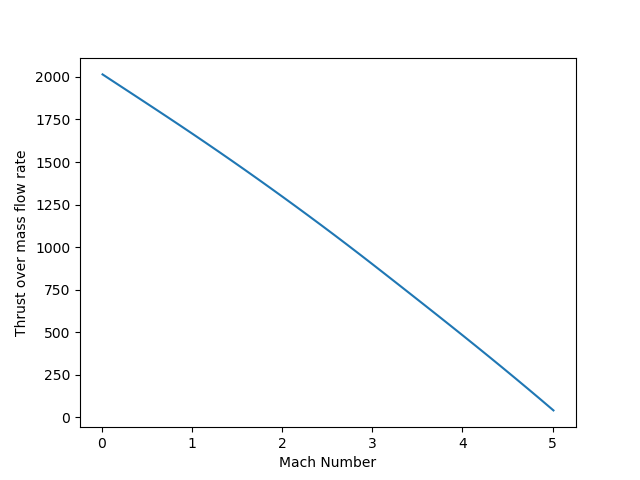
\includegraphics[width=0.9\textwidth]{propan_pow(1mol)/Thrust_over_mass_flow_rate_over_Mach.png}
       		\caption{Thrust over mass flow rate over Mach number for propane-air mixture}
	\end{figure}
	\begin{figure}[H]
		\centering
		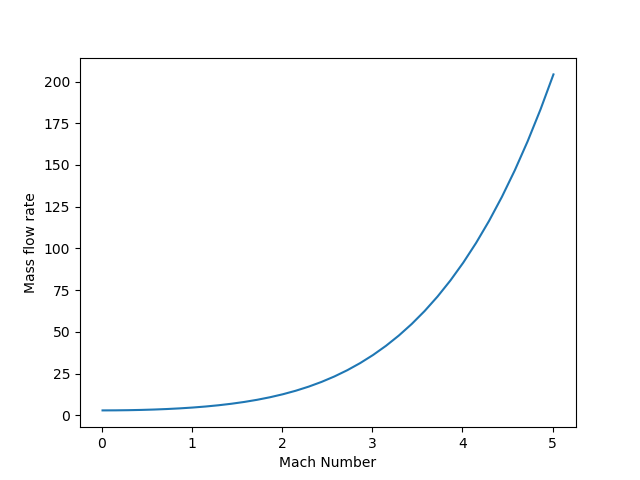
\includegraphics[width=0.9\textwidth]{propan_pow(1mol)/Mass_flow_rate_over_Mach.png}
       		\caption{Mass flow rate over Mach number for propane-air mixture}
	\end{figure}
\subsection{Hydrogen - air mixture}
	\begin{figure}[H]
		\centering
       		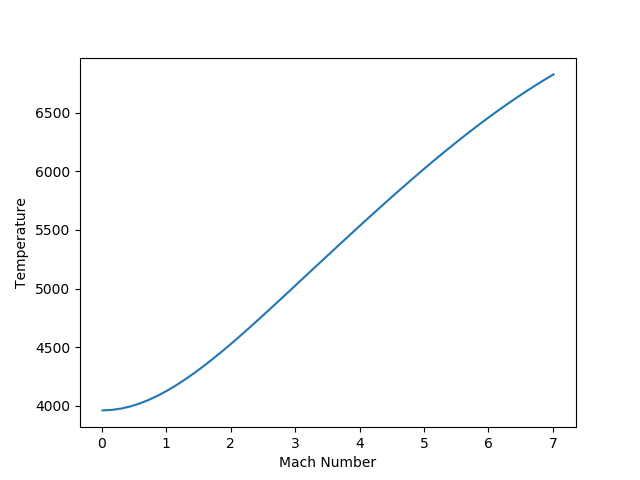
\includegraphics[width=0.9\textwidth]{H2_pow(1mol)/Temperature_over_Mach.png}
       		\caption{Temperature over Mach number for hydrogen-air mixture}
	\end{figure}
	\begin{figure}[H]
		\centering
		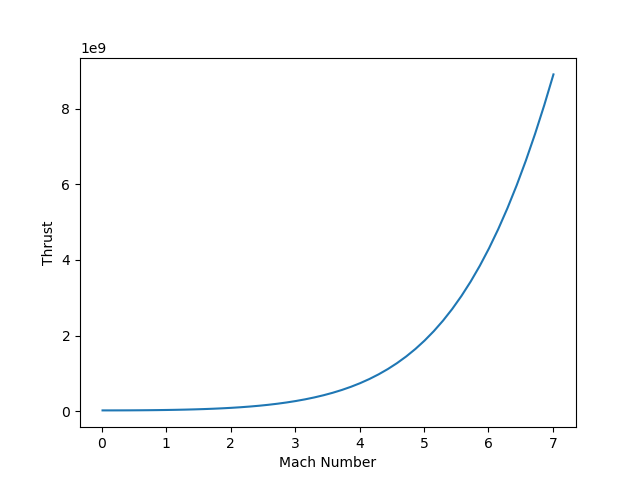
\includegraphics[width=0.9\textwidth]{H2_pow(1mol)/Thrust_over_Mach.png}
       		\caption{Thrust over Mach number for hydrogen-air mixture}
	\end{figure}
	\begin{figure}[H]
		\centering
		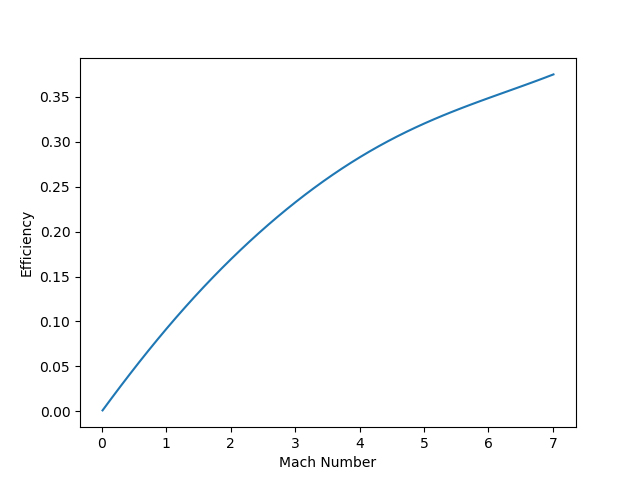
\includegraphics[width=0.9\textwidth]{H2_pow(1mol)/Efficiency_over_Mach.png}
       		\caption{Efficiency over Mach number for hydrogen-air mixture}
	\end{figure}
	\begin{figure}[H]
		\centering
		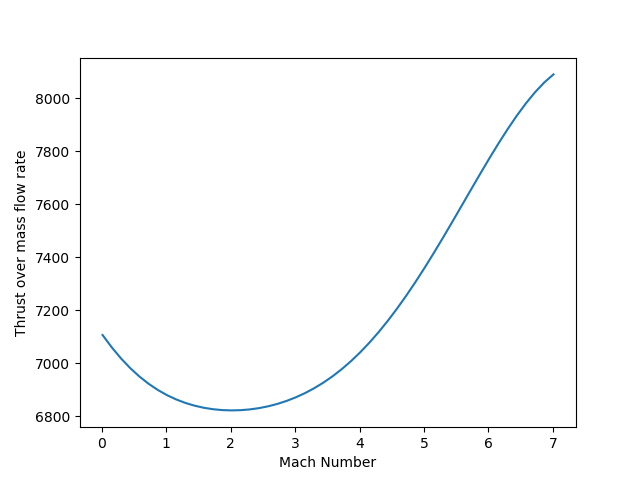
\includegraphics[width=0.9\textwidth]{H2_pow(1mol)/Thrust_over_mass_flow_rate_over_Mach.png}
       		\caption{Thrust over mass flow rate over Mach number for hydrogen-air mixture}
	\end{figure}
	\begin{figure}[H]
		\centering
		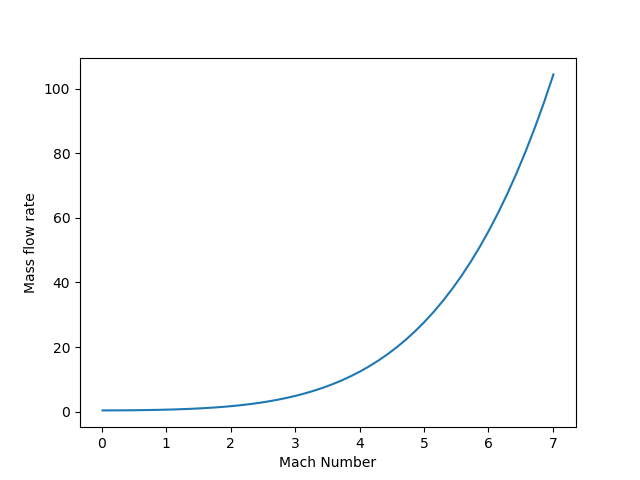
\includegraphics[width=0.9\textwidth]{H2_pow(1mol)/Mass_flow_rate_over_Mach.png}
       		\caption{Mass flow rate over Mach number for hydrogen-air mixture}
	\end{figure}
\subsection{Methane (1 mol) - ethane (0.4 mol) - air mixture}
	\begin{figure}[H]
		\centering
       		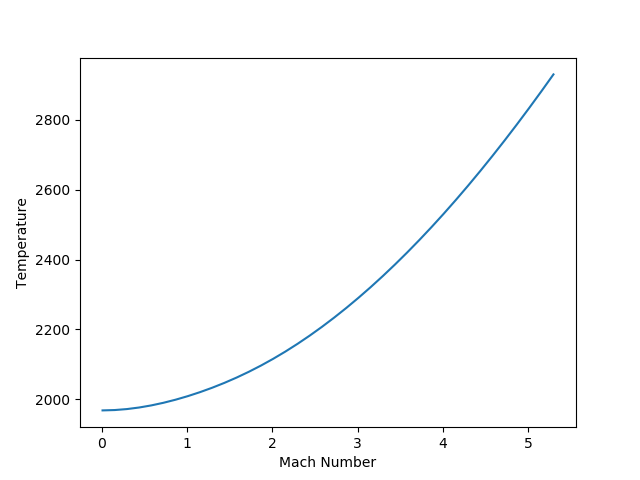
\includegraphics[width=0.9\textwidth]{metan(1mol)_etan(0.4mol)_pow/Temperature_over_Mach.png}
       		\caption{Temperature over Mach number for methane-ethane-air mixture}
	\end{figure}
	\begin{figure}[H]
		\centering
		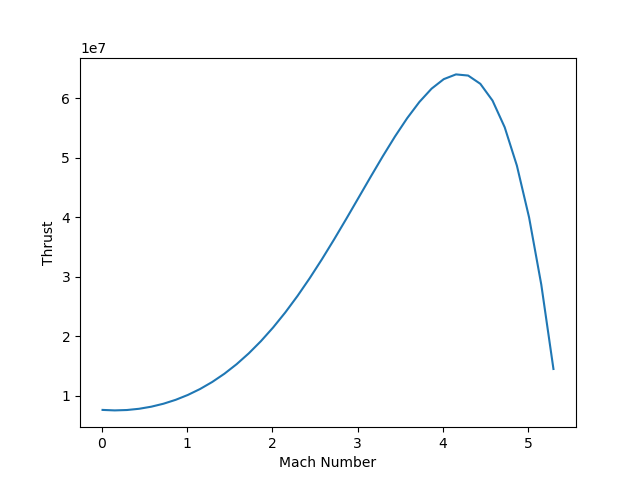
\includegraphics[width=0.9\textwidth]{metan(1mol)_etan(0.4mol)_pow/Thrust_over_Mach.png}
       		\caption{Thrust over Mach number for methane-ethane-air mixture}
	\end{figure}
	\begin{figure}[H]
		\centering
		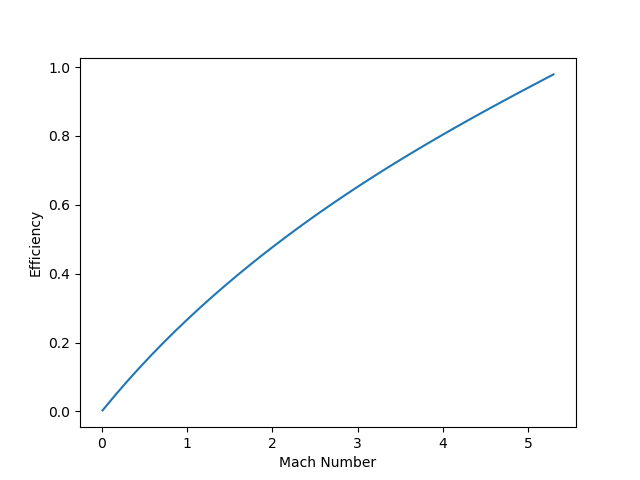
\includegraphics[width=0.9\textwidth]{metan(1mol)_etan(0.4mol)_pow/Efficiency_over_Mach.png}
       		\caption{Efficiency over Mach number for methane-ethane-air mixture}
	\end{figure}
	\begin{figure}[H]
		\centering
		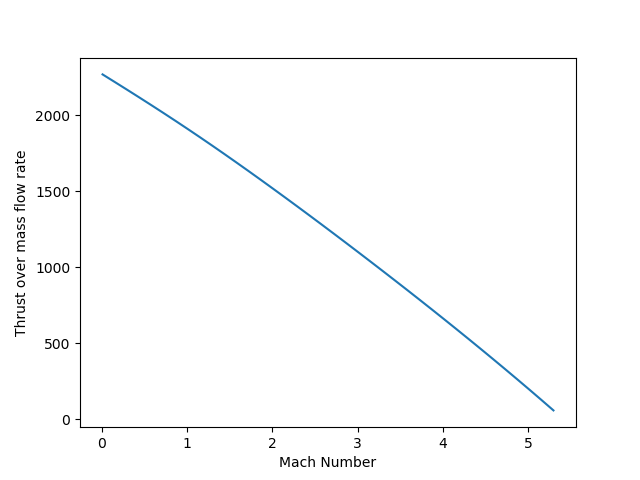
\includegraphics[width=0.9\textwidth]{metan(1mol)_etan(0.4mol)_pow/Thrust_over_mass_flow_rate_over_Mach.png}
       		\caption{Thrust over mass flow rate over Mach number for methane-ethane-air mixture}
	\end{figure}
	\begin{figure}[H]
		\centering
		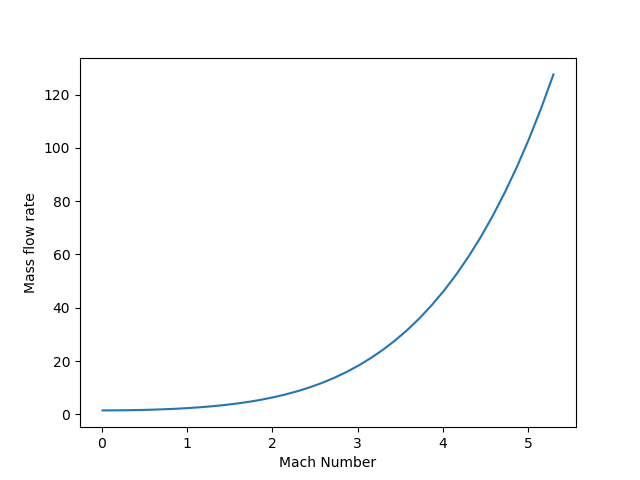
\includegraphics[width=0.9\textwidth]{metan(1mol)_etan(0.4mol)_pow/Mass_flow_rate_over_Mach.png}
       		\caption{Mass flow rate over Mach number for methane-ethane-air mixture}
	\end{figure}
\subsection{Methane (2 mol) - propane (1 mol) - air mixture}
	\begin{figure}[H]
		\centering
       		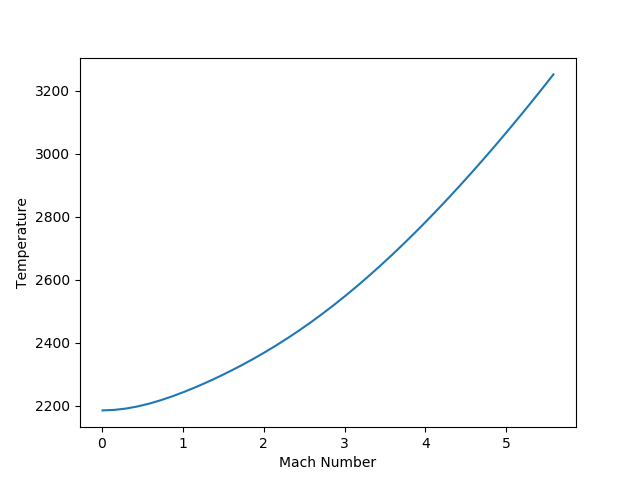
\includegraphics[width=0.9\textwidth]{Metan(2mol)_propan(1mol)_pow/Temperature_over_Mach.png}
       		\caption{Temperature over Mach number for methane-propane-air mixture}
	\end{figure}
	\begin{figure}[H]
		\centering
		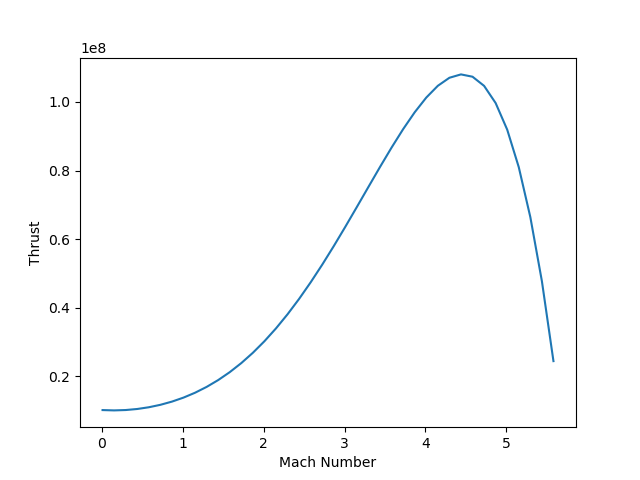
\includegraphics[width=0.9\textwidth]{Metan(2mol)_propan(1mol)_pow/Thrust_over_Mach.png}
       		\caption{Thrust over Mach number for methane-propane-air mixture}
	\end{figure}
	\begin{figure}[H]
		\centering
		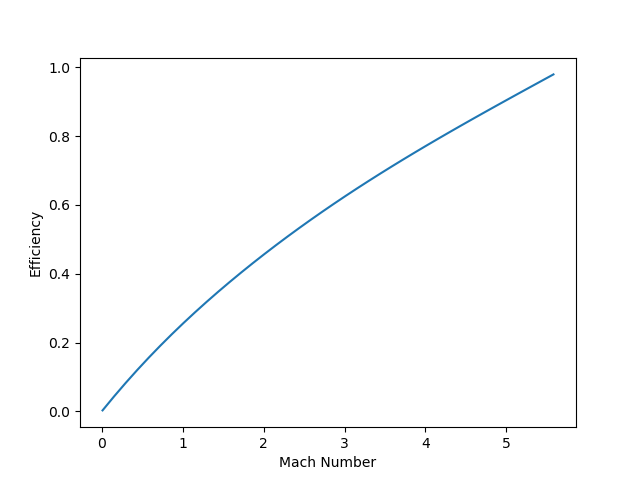
\includegraphics[width=0.9\textwidth]{Metan(2mol)_propan(1mol)_pow/Efficiency_over_Mach.png}
       		\caption{Efficiency over Mach number for methane-propane-air mixture}
	\end{figure}
	\begin{figure}[H]
		\centering
		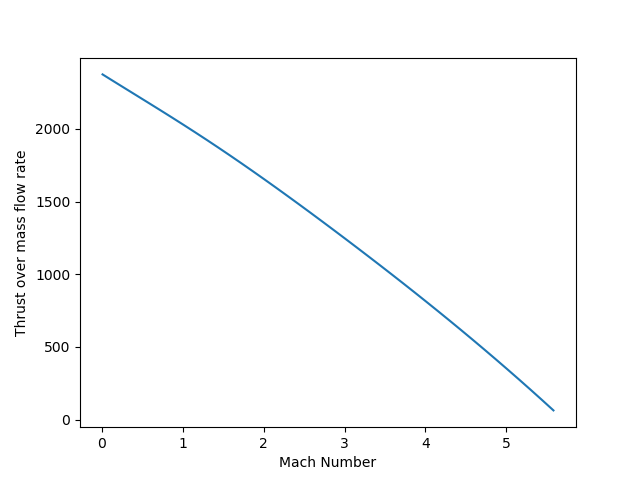
\includegraphics[width=0.9\textwidth]{Metan(2mol)_propan(1mol)_pow/Thrust_over_mass_flow_rate_over_Mach.png}
       		\caption{Thrust over mass flow rate over Mach number for methane-propane-air mixture}
	\end{figure}
	\begin{figure}[H]
		\centering
		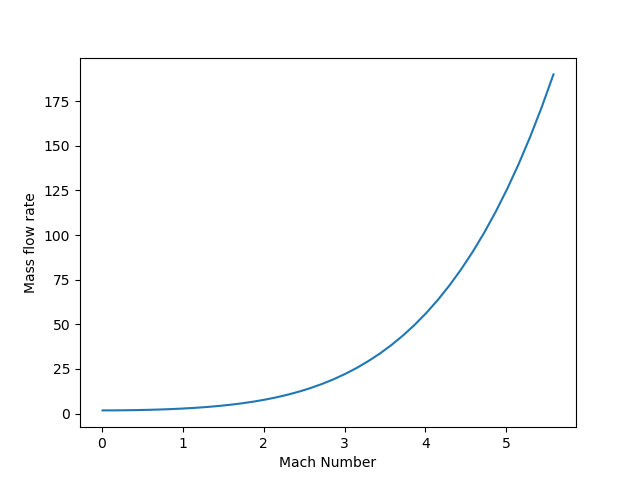
\includegraphics[width=0.9\textwidth]{Metan(2mol)_propan(1mol)_pow/Mass_flow_rate_over_Mach.png}
       		\caption{Mass flow rate over Mach number for methane-propane-air mixture}
	\end{figure}
\subsection{Ethane (1 mol) - hydrogen (0.5 mol) - air mixture}
	\begin{figure}[H]
		\centering
       		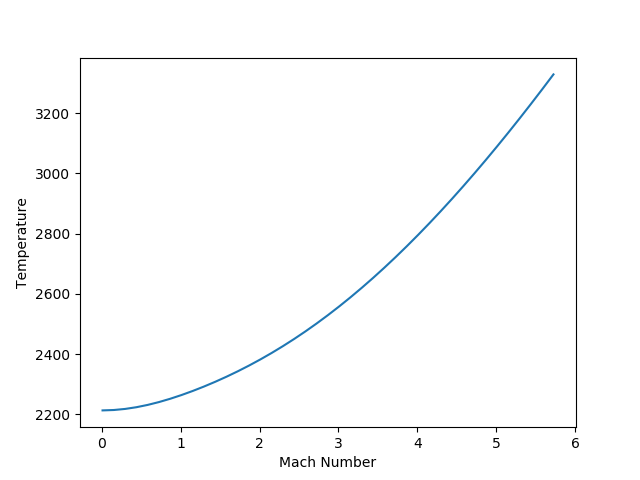
\includegraphics[width=0.9\textwidth]{Wodor(0.5mol)_Etan(1mol)_pow/Temperature_over_Mach.png}
       		\caption{Temperature over Mach number for ethane-hydrogen-air mixture}
	\end{figure}
	\begin{figure}[H]
		\centering
		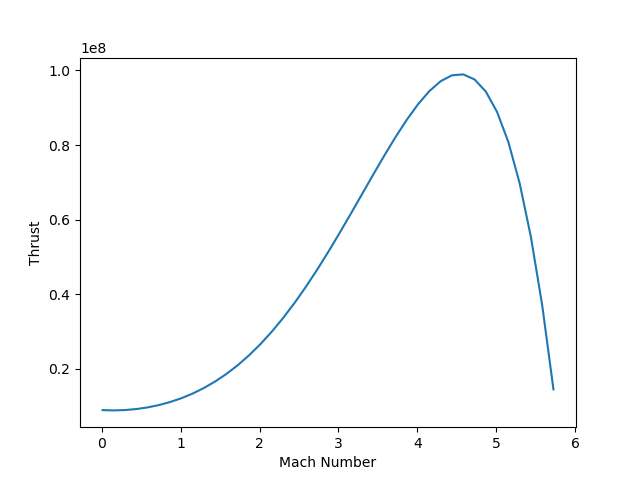
\includegraphics[width=0.9\textwidth]{Wodor(0.5mol)_Etan(1mol)_pow/Thrust_over_Mach.png}
       		\caption{Thrust over Mach number for ethane-hydrogen-air mixture}
	\end{figure}
	\begin{figure}[H]
		\centering
		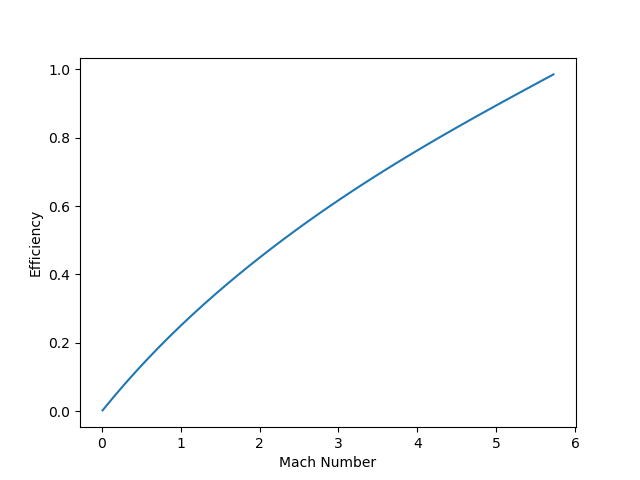
\includegraphics[width=0.9\textwidth]{Wodor(0.5mol)_Etan(1mol)_pow/Efficiency_over_Mach.png}
       		\caption{Efficiency over Mach number for ethane-hydrogen-air mixture}
	\end{figure}
	\begin{figure}[H]
		\centering
		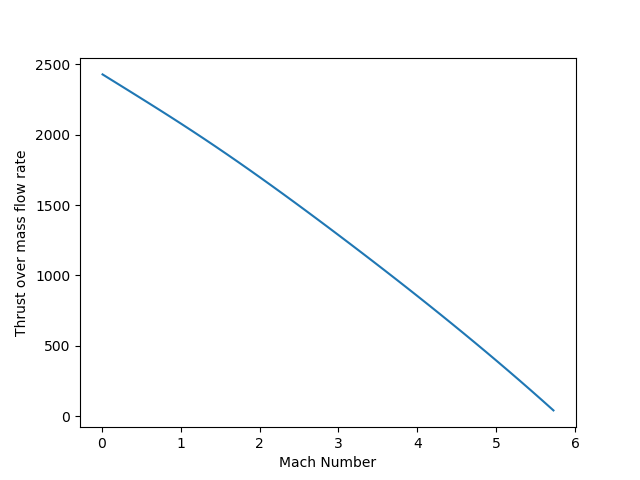
\includegraphics[width=0.9\textwidth]{Wodor(0.5mol)_Etan(1mol)_pow/Thrust_over_mass_flow_rate_over_Mach.png}
       		\caption{Thrust over mass flow rate over Mach number for ethane-hydrogen-air mixture}
	\end{figure}
	\begin{figure}[H]
		\centering
		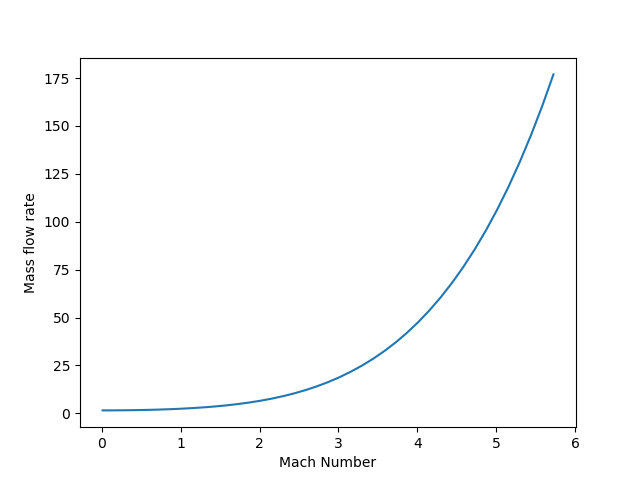
\includegraphics[width=0.9\textwidth]{Wodor(0.5mol)_Etan(1mol)_pow/Mass_flow_rate_over_Mach.png}
       		\caption{Mass flow rate over Mach number for ethane-hydrogen-air mixture}
	\end{figure}
\subsection{Propane (1 mol) - hydrogen (0.1 mol) - air mixture}
	\begin{figure}[H]
		\centering
       		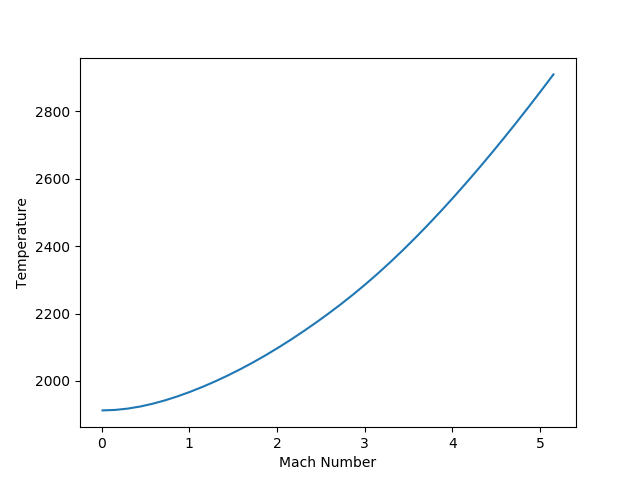
\includegraphics[width=0.9\textwidth]{Propan(1mol)_wodor(0.1mol)_pow/Temperature_over_Mach.png}
       		\caption{Temperature over Mach number for propane-hydrogen-air mixture}
	\end{figure}
	\begin{figure}[H]
		\centering
		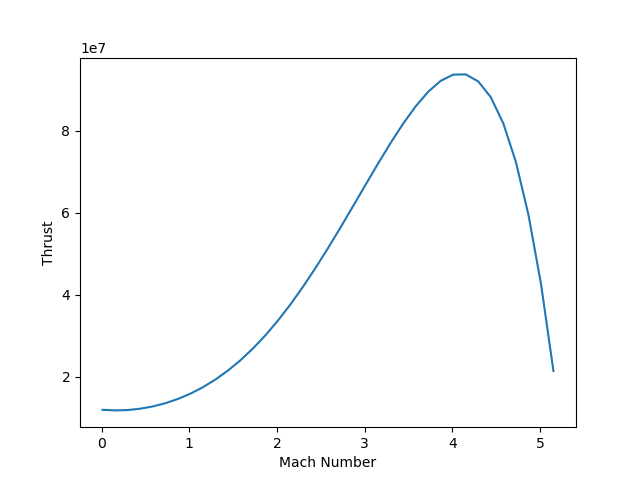
\includegraphics[width=0.9\textwidth]{Propan(1mol)_wodor(0.1mol)_pow/Thrust_over_Mach.png}
       		\caption{Thrust over Mach number for propane-hydrogen-air mixture}
	\end{figure}
	\begin{figure}[H]
		\centering
		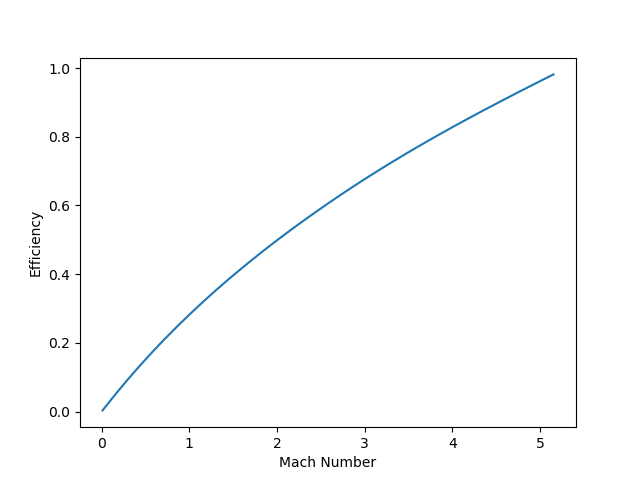
\includegraphics[width=0.9\textwidth]{Propan(1mol)_wodor(0.1mol)_pow/Efficiency_over_Mach.png}
       		\caption{Efficiency over Mach number for propane-hydrogen-air mixture}
	\end{figure}
	\begin{figure}[H]
		\centering
		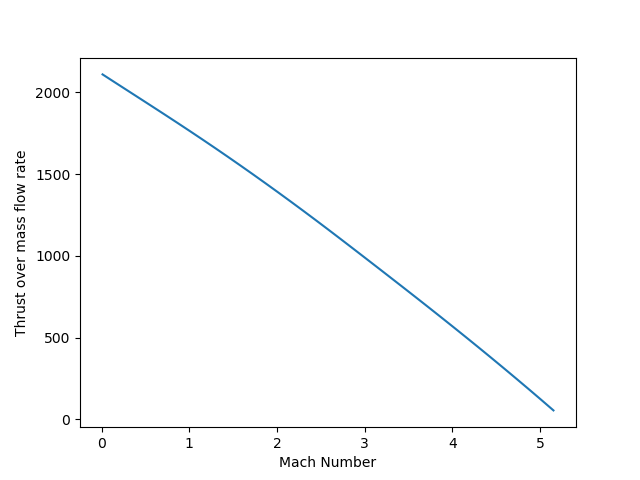
\includegraphics[width=0.9\textwidth]{Propan(1mol)_wodor(0.1mol)_pow/Thrust_over_mass_flow_rate_over_Mach.png}
       		\caption{Thrust over mass flow rate over Mach number for propane-hydrogen-air mixture}
	\end{figure}
	\begin{figure}[H]
		\centering
		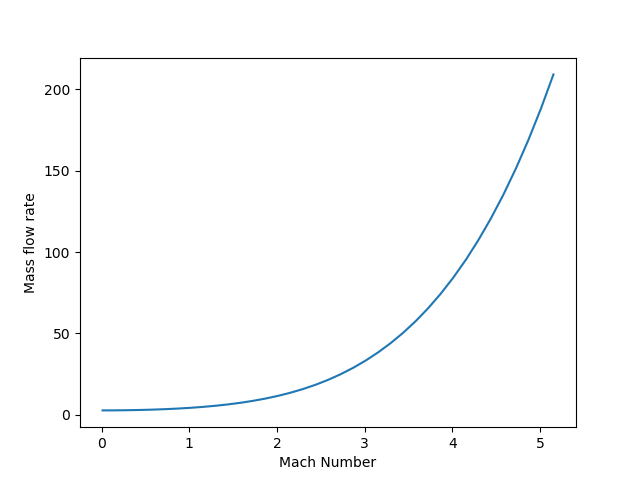
\includegraphics[width=0.9\textwidth]{Propan(1mol)_wodor(0.1mol)_pow/Mass_flow_rate_over_Mach.png}
       		\caption{Mass flow rate over Mach number for propane-hydrogen-air mixture}
	\end{figure}
\subsection{Methane (1 mol) - ethane (0.4 mol) - propane (0.2 mol) - air mixture}
	\begin{figure}[H]
		\centering
       		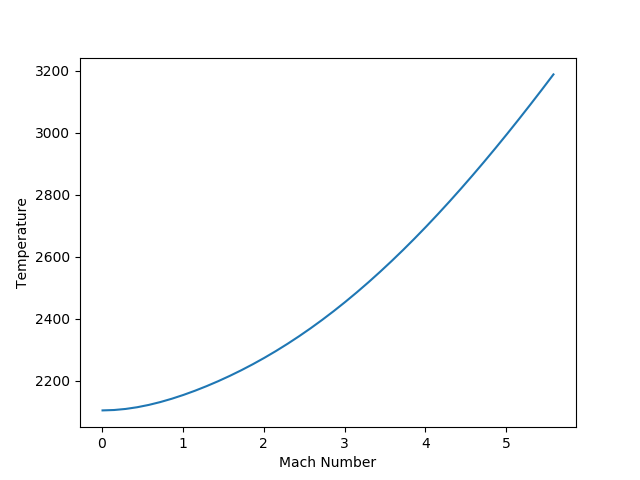
\includegraphics[width=0.9\textwidth]{Metan(1mol)_etan(0.4mol)_propan(0.2mol)_pow/Temperature_over_Mach.png}
       		\caption{Temperature over Mach number for methane-ethane-propane-air mixture}
	\end{figure}
	\begin{figure}[H]
		\centering
		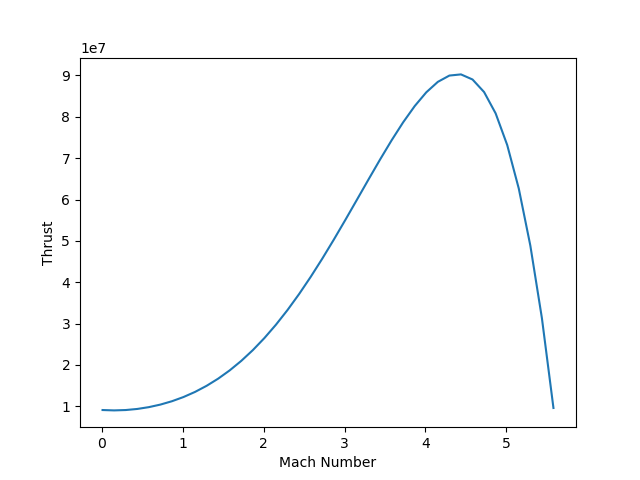
\includegraphics[width=0.9\textwidth]{Metan(1mol)_etan(0.4mol)_propan(0.2mol)_pow/Thrust_over_Mach.png}
       		\caption{Thrust over Mach number for methane-ethane-propane-air mixture}
	\end{figure}
	\begin{figure}[H]
		\centering
		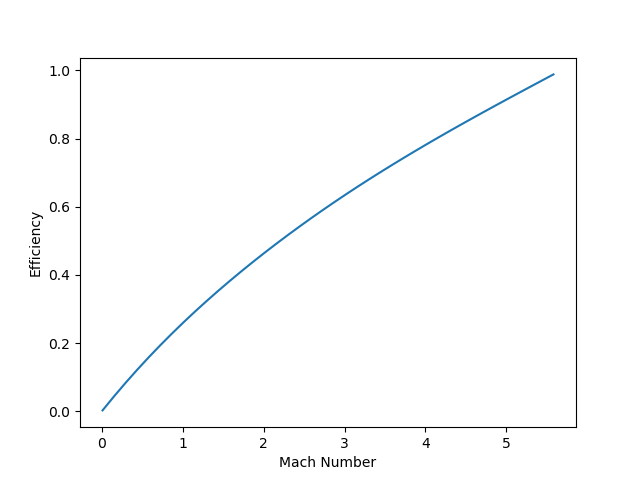
\includegraphics[width=0.9\textwidth]{Metan(1mol)_etan(0.4mol)_propan(0.2mol)_pow/Efficiency_over_Mach.png}
       		\caption{Efficiency over Mach number for methane-ethane-propane-air mixture}
	\end{figure}
	\begin{figure}[H]
		\centering
		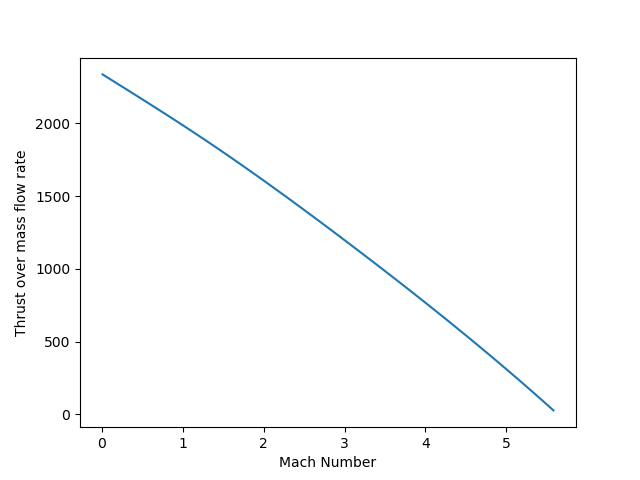
\includegraphics[width=0.9\textwidth]{Metan(1mol)_etan(0.4mol)_propan(0.2mol)_pow/Thrust_over_mass_flow_rate_over_Mach.png}
       		\caption{Thrust over mass flow rate over Mach number for methane-ethane-propane-air mixture}
	\end{figure}
	\begin{figure}[H]
		\centering
		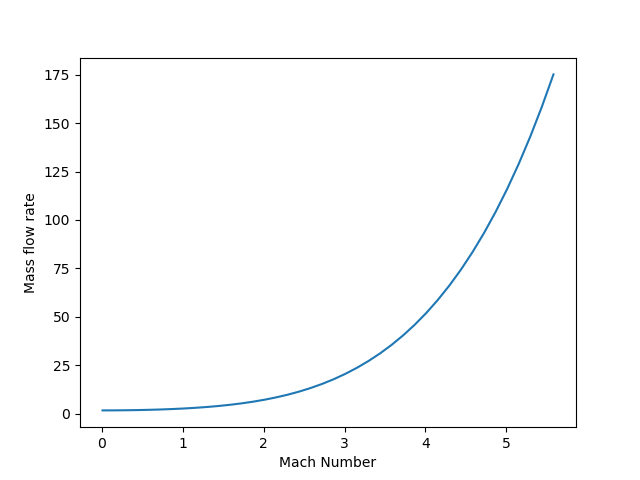
\includegraphics[width=0.9\textwidth]{Metan(1mol)_etan(0.4mol)_propan(0.2mol)_pow/Mass_flow_rate_over_Mach.png}
       		\caption{Mass flow rate over Mach number for methane-ethane-propane-air mixture}
	\end{figure}

\section{Summary}

The results show that the maximum thrust does not coincide with the highest temperature in the combustion chamber. Particularly interesting is also maximum thrust achievable for each mixture. Performed calculations show clearly, that hydrogen-air stoichiometric mixture can achieve much higher thrust than any other tested mixture. Another thing is that for each mixture, except hydrogen-air, the thrust drops as Mach number increases. In our calculation range (i. e. for maximum Mach number equal to 7) for hydrogen-air mixture the thrust increases as Mach number increases. For that mixture highest thrust comes also with highest temperature, which maximum value is equal to about 6900 K. For other mixtures it is also clearly visible that achieved thrust is associated with temperature in combustion chamber.

As mentioned earlier, for each mixture, except hydrogen-air, thrust drops and approaches zero with increase of Mach number. The explanation of this phenomenon is as follows: for a certain area of inlet, fuel and equivalence ratio the engine can opearate up to a boundary Mach number. That boundary value can be obtained from the formula for specific thrust:

$$v_e-v_0=v_e-a*Ma$$
As the growth of temperature is slower than growth of inlet velocity, the specific thrust approaches zero.

\end{document}